\documentclass[a4paper,11pt]{article}
\usepackage{amssymb,amsthm}
\usepackage{amsmath}
\usepackage{setspace}

\usepackage{adjustbox}
\usepackage{graphicx}
\usepackage[margin=1in]{geometry}
\usepackage{mathtools}
\usepackage{qtree}
\usepackage{tikz}
\usetikzlibrary{automata,positioning,decorations.markings,arrows}

\usepackage{xcolor}

\begin{document}
\begin{center}
{\large{ASSIGNMENT-2\\
COMPUTER NETWORK}}
\end{center}
\begin{enumerate}

\item[Q1.]
 Hosts A and B are each connected  via two routers $R_1$ and $R_2$  and a with 10$^{8}$ bits per second links. Each link has a
propagation delay of 120 microseconds. Processing delay at router is 500 microseconds . \\

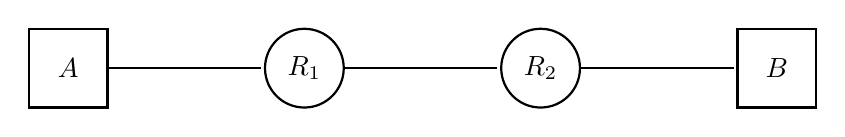
\begin{tikzpicture}[->,>=stealth',shorten >=1pt,auto,node distance=3cm,
        thick,main node/.style={rectangle ,draw,minimum size=1cm,inner sep=0pt]}]

    \node[main node] (1) {$A$};
    \node[main node][circle] (2) [right of=1]  {$R_1$};
    \node[main node][circle] (3) [ right of=2] {$R_2$};
 \node[main node] (4) [right of=3] {$B$};

    \path[-]
    (1) edge node {} (2)

    (2)
        edge node {} (3)
        (3)
        edge node {} (4)
        ;

\end{tikzpicture}\\

   If message size is 10 KB.Calculate the time elapsed between the transmission of the
first bit of data and the reception of the last bit of the data in the following cases :
\begin{enumerate}
  \item If message switching technique is used.
  \item Assume packet header size is negligible
  \begin{enumerate}
  \item If packet switching technique is used and 8 packets of same size are used
  \item If packet switching technique is used and 32 packets of same size are used
      \item If packet switching technique is used and 64 packets of same size are used
\end{enumerate}
\item Assume packet header size is 200 bits
\begin{enumerate}
  \item If packet switching technique is used and 8 packets of same size are used
  \item If packet switching technique is used and 32 packets of same size are used
      \item If packet switching technique is used and 64 packets of same size are used
\end{enumerate}
 \end{enumerate}
\item[Q2.]
 Hosts A and B are each connected  via three routers $R_1$ , $R_2$ and $R_3$ and a with 5MBps links. Each link has a
propagation delay of 500 millisecond/KM. Processing delay at router is 500 microseconds . \\

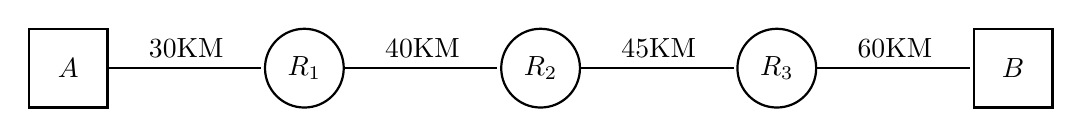
\begin{tikzpicture}[->,>=stealth',shorten >=1pt,auto,node distance=3cm,
        thick,main node/.style={rectangle ,draw,minimum size=1cm,inner sep=0pt]}]

    \node[main node] (1) {$A$};
    \node[main node][circle] (2) [right of=1]  {$R_1$};
    \node[main node][circle] (3) [ right of=2] {$R_2$};
    \node[main node][circle] (5) [ right of=3] {$R_3$};
 \node[main node] (4) [right of=5] {$B$};

    \path[-]
    (1) edge node {30KM} (2)

    (2)
        edge node {40KM} (3)
        (3)
        edge node {45KM} (5)
        (5)
        edge node {60KM} (4)
        ;

\end{tikzpicture}\\

   If message size is 8192 bits .Calculate the time elapsed between the transmission of the
first bit of data and the reception of the last bit of the data in the following cases :
\begin{enumerate}
  \item If message switching technique is used.
  \item Assume packet header size is negligible
  \begin{enumerate}
  \item If packet switching technique is used and 4 packets of same size are used
  \item If packet switching technique is used and 16 packets of same size are used
      \item If packet switching technique is used and 32 packets of same size are used
\end{enumerate}
\item Assume packet header size is 100 bits
\begin{enumerate}
  \item If packet switching technique is used and 4 packets of same size are used
  \item If packet switching technique is used and 16 packets of same size are used
      \item If packet switching technique is used and 64 packets of same size are used
\end{enumerate}

 \end{enumerate}



\item[Q3.]
 Hosts A and B are each connected  via  router $R_1$  and a with 5MBps links. Each link has a
propagation delay of 5 milliseconds/KM. Processing delay at router is 400 milliseconds . \\

\begin{tikzpicture}[->,>=stealth',shorten >=1pt,auto,node distance=3cm,
        thick,main node/.style={rectangle ,draw,minimum size=1cm,inner sep=0pt]}]

    \node[main node] (1) {$A$};
    \node[main node][circle] (2) [right of=1]  {$R_1$};

 \node[main node] (4) [right of=2] {$B$};

    \path[-]
    (1) edge node {30KM} (2)

    (2)
        edge node {40KM} (3)
        (3)

        ;

\end{tikzpicture}\\

   If message size is 100KB  .Calculate the time elapsed between the transmission of the
first bit of data and the reception of the last bit of the data in the following cases :
\begin{enumerate}
  \item If message switching technique is used.
  \item Assume packet header size is negligible
  \begin{enumerate}
  \item If packet switching technique is used and 4 packets of same size are used
  \item If packet switching technique is used and 64 packets of same size are used
      \item If packet switching technique is used and 128 packets of same size are used(if possible)
\end{enumerate}
\item Assume packet header size is 400 bits
\begin{enumerate}
  \item If packet switching technique is used and 4 packets of same size are used
  \item If packet switching technique is used and 64 packets of same size are used
      \item If packet switching technique is used and 128 packets of same size are used(if possible)
\end{enumerate}

 \end{enumerate}




\item[Q4.]
 Hosts A and B are each connected  via two routers $R_1$ and $R_2$  and a with 10MBPS links. Each link has a
propagation delay of 220 microseconds. Processing delay at router is 600 microseconds . \\

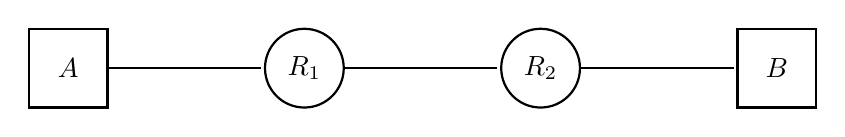
\begin{tikzpicture}[->,>=stealth',shorten >=1pt,auto,node distance=3cm,
        thick,main node/.style={rectangle ,draw,minimum size=1cm,inner sep=0pt]}]

    \node[main node] (1) {$A$};
    \node[main node][circle] (2) [right of=1]  {$R_1$};
    \node[main node][circle] (3) [ right of=2] {$R_2$};
 \node[main node] (4) [right of=3] {$B$};

    \path[-]
    (1) edge node {} (2)

    (2)
        edge node {} (3)
        (3)
        edge node {} (4)
        ;

\end{tikzpicture}\\

   If message size is 10 KB.Calculate the time elapsed between the transmission of the
first bit of data and the reception of the last bit of the data in the following cases :
\begin{enumerate}
  \item If message switching technique is used.
  \item Assume packet header size is negligible
  \begin{enumerate}
  \item If packet switching technique is used and Packet size is 1500 bits
  \item If packet switching technique is used and Packet size is 1000 bits
      \item If packet switching technique is used and Packet size is 2500 bits
\end{enumerate}
\item Assume packet header size is 200 bits
\begin{enumerate}
   \item If packet switching technique is used and Packet size is 1500 bits
  \item If packet switching technique is used and Packet size is 1000 bits
      \item If packet switching technique is used and Packet size is 2500 bits
\end{enumerate}
 \end{enumerate}
\item[Q5.]
 Hosts A and B are each connected  via three routers $R_1$ , $R_2$ and $R_3$ and a with 5MBps links. Each link has a
propagation delay of 500 millisecond/KM. Processing delay at router is 500 microseconds . \\

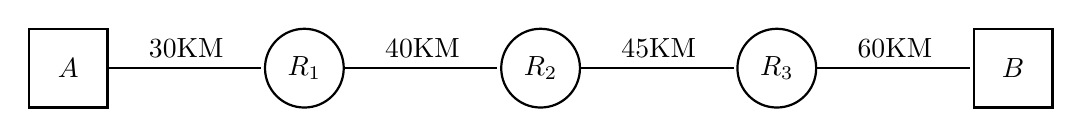
\begin{tikzpicture}[->,>=stealth',shorten >=1pt,auto,node distance=3cm,
        thick,main node/.style={rectangle ,draw,minimum size=1cm,inner sep=0pt]}]

    \node[main node] (1) {$A$};
    \node[main node][circle] (2) [right of=1]  {$R_1$};
    \node[main node][circle] (3) [ right of=2] {$R_2$};
    \node[main node][circle] (5) [ right of=3] {$R_3$};
 \node[main node] (4) [right of=5] {$B$};

    \path[-]
    (1) edge node {30KM} (2)

    (2)
        edge node {40KM} (3)
        (3)
        edge node {45KM} (5)
        (5)
        edge node {60KM} (4)
        ;

\end{tikzpicture}\\

   If message size is 100KB .Calculate the time elapsed between the transmission of the
first bit of data and the reception of the last bit of the data in the following cases :
\begin{enumerate}
  \item If message switching technique is used.
  \item Assume packet header size is negligible
  \begin{enumerate}
  \item If packet switching technique is used and Packet size is 1000 bits
  \item If packet switching technique is used and Packet size is 2000 bits
      \item If packet switching technique is used and Packet size is 3000 bits
\end{enumerate}
\item Assume packet header size is 200 bits
\begin{enumerate}
   \item If packet switching technique is used and Packet size is 1000 bits
  \item If packet switching technique is used and Packet size is 2000 bits
      \item If packet switching technique is used and Packet size is 3000 bits
\end{enumerate}
 \end{enumerate}



\item[Q6.]
 Hosts A and B are each connected  via  router $R_1$  and a with 5MBps links. Each link has a
propagation delay of 5 milliseconds/KM. Processing delay at router is 400 milliseconds . \\

\begin{tikzpicture}[->,>=stealth',shorten >=1pt,auto,node distance=3cm,
        thick,main node/.style={rectangle ,draw,minimum size=1cm,inner sep=0pt]}]

    \node[main node] (1) {$A$};
    \node[main node][circle] (2) [right of=1]  {$R_1$};

 \node[main node] (4) [right of=2] {$B$};

    \path[-]
    (1) edge node {30KM} (2)

    (2)
        edge node {40KM} (3)
        (3)

        ;

\end{tikzpicture}\\

   If message size is 100KB  .Calculate the time elapsed between the transmission of the
first bit of data and the reception of the last bit of the data in the following cases :
\begin{enumerate}
  \item If message switching technique is used.
  \item Assume packet header size is negligible
  \begin{enumerate}
  \item If packet switching technique is used and Packet size is 100 bits
  \item If packet switching technique is used and Packet size is 800 bits
      \item If packet switching technique is used and Packet size is 2200 bits
\end{enumerate}
\item Assume packet header size is 200 bits
\begin{enumerate}
   \item If packet switching technique is used and Packet size is 800 bits
  \item If packet switching technique is used and Packet size is 1200 bits
      \item If packet switching technique is used and Packet size is 2400 bits
\end{enumerate}
 \end{enumerate}

\item[Q7.]
 Hosts A and B are each connected  via two routers $R_1$ and $R_2$. Each link has a
propagation delay of 220 microseconds. Processing delay at router is 600 microseconds . Bandwidth of each link is denoted by K , S and R in following diagram \\

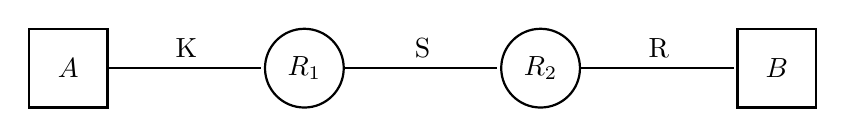
\begin{tikzpicture}[->,>=stealth',shorten >=1pt,auto,node distance=3cm,
        thick,main node/.style={rectangle ,draw,minimum size=1cm,inner sep=0pt]}]

    \node[main node] (1) {$A$};
    \node[main node][circle] (2) [right of=1]  {$R_1$};
    \node[main node][circle] (3) [ right of=2] {$R_2$};
 \node[main node] (4) [right of=3] {$B$};

    \path[-]
    (1) edge node {K} (2)

    (2)
        edge node {S} (3)
        (3)
        edge node {R} (4)
        ;

\end{tikzpicture}\\

   If message size is 100 KB.Calculate the time elapsed between the transmission of the
first bit of data and the reception of the last bit of the data in the following cases :
\begin{enumerate}
 \item if value of K,S and R is 10Mbps, 20Mbps , 30Mbps respectively
\begin{enumerate}
  \item If message switching technique is used.
  \item Assume packet header size is negligible
  \begin{enumerate}
   \item If packet switching technique is used and Packet size is 8000 bits

      \item If packet switching technique is used and Packet size is 12000 bits
\end{enumerate}
\item Assume packet header size is 800 bits
\begin{enumerate}
   \item If packet switching technique is used and Packet size is 8000 bits

      \item If packet switching technique is used and Packet size is 12000 bits
\end{enumerate}
 \end{enumerate}
 \item if value of K,S and R is 30Mbps, 20Mbps , 10Mbps respectively
\begin{enumerate}
  \item If message switching technique is used.
  \item Assume packet header size is negligible
  \begin{enumerate}
    \item If packet switching technique is used and Packet size is 8000 bits

      \item If packet switching technique is used and Packet size is 12000 bits
\end{enumerate}
\item Assume packet header size is 800 bits
\begin{enumerate}
   \item If packet switching technique is used and Packet size is 8000 bits

      \item If packet switching technique is used and Packet size is 12000 bits
\end{enumerate}
 \end{enumerate}

 \item if value of K,S and R is 20Mbps, 10Mbps , 30Mbps respectively
\begin{enumerate}
  \item If message switching technique is used.
  \item Assume packet header size is negligible
  \begin{enumerate}
    \item If packet switching technique is used and Packet size is 8000 bits

      \item If packet switching technique is used and Packet size is 12000 bits
\end{enumerate}
\item Assume packet header size is 800 bits
\begin{enumerate}
   \item If packet switching technique is used and Packet size is 8000 bits

      \item If packet switching technique is used and Packet size is 12000 bits
\end{enumerate}
 \end{enumerate}
 \end{enumerate}


\item[Q8.]
 Hosts A and B are each connected  via two routers $R_1$ and $R_2$. Each link has a
propagation delay of 620 microseconds. Processing delay at router is 400 microseconds . Bandwidth of each link is denoted by K , S and R in following diagram \\

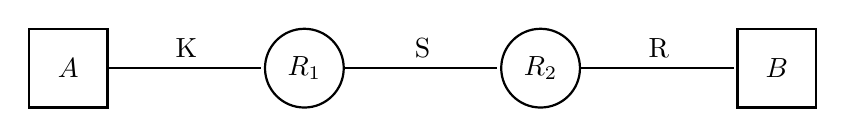
\begin{tikzpicture}[->,>=stealth',shorten >=1pt,auto,node distance=3cm,
        thick,main node/.style={rectangle ,draw,minimum size=1cm,inner sep=0pt]}]

    \node[main node] (1) {$A$};
    \node[main node][circle] (2) [right of=1]  {$R_1$};
    \node[main node][circle] (3) [ right of=2] {$R_2$};
 \node[main node] (4) [right of=3] {$B$};

    \path[-]
    (1) edge node {K} (2)

    (2)
        edge node {S} (3)
        (3)
        edge node {R} (4)
        ;

\end{tikzpicture}\\

   If message size is 120 KB.Calculate the time elapsed between the transmission of the
first bit of data and the reception of the last bit of the data in the following cases :
\begin{enumerate}
 \item if value of K,S and R is 5Mbps, 10Mbps , 15Mbps respectively
\begin{enumerate}
  \item If message switching technique is used.
  \item Assume packet header size is negligible
  \begin{enumerate}
   \item If packet switching technique is used and Packet size is 5000 bits

      \item If packet switching technique is used and Packet size is 7000 bits
\end{enumerate}
\item Assume packet header size is 800 bits
\begin{enumerate}
   \item If packet switching technique is used and Packet size is 5000 bits

      \item If packet switching technique is used and Packet size is 7000 bits
\end{enumerate}
 \end{enumerate}
 \item if value of K,S and R is 10Mbps, 5Mbps , 15Mbps respectively
\begin{enumerate}
  \item If message switching technique is used.
  \item Assume packet header size is negligible
  \begin{enumerate}
    \item If packet switching technique is used and Packet size is 5000 bits

      \item If packet switching technique is used and Packet size is 7000 bits
\end{enumerate}
\item Assume packet header size is 800 bits
\begin{enumerate}
   \item If packet switching technique is used and Packet size is 5000 bits

      \item If packet switching technique is used and Packet size is 7000 bits
\end{enumerate}
 \end{enumerate}

 \item if value of K,S and R is 15Mbps, 10Mbps , 5Mbps respectively
\begin{enumerate}
  \item If message switching technique is used.
  \item Assume packet header size is negligible
  \begin{enumerate}
    \item If packet switching technique is used and Packet size is 5000 bits

      \item If packet switching technique is used and Packet size is 7000 bits
\end{enumerate}
\item Assume packet header size is 800 bits
\begin{enumerate}
   \item If packet switching technique is used and Packet size is 5000 bits

      \item If packet switching technique is used and Packet size is 7000 bits
\end{enumerate}
 \end{enumerate}
 \end{enumerate}

\item[Q9.]
In a network , two Host A and B tries to send the data and in case of collision, random amount of time is being calculated by binary back-off algorithm.Assume following operations are being carried out in sequence
\begin{itemize}
  \item  Data sent by A and B collides for 3 times in sequence
  \item A successfully send the data
  \item Data sent by A and B collides for 2 times in sequence
  \item B successfully send the data
  \item Data sent by A and B collides for 2 times in sequence
\end{itemize}
Answer the Followings
\begin{enumerate}
  \item What is the probability of collision
  \item What is the probability that A win the backoff race
  \item What is the probability that B win the backoff race
\end{enumerate}

\item[Q10.]
In a network , two Host A and B tries to send the data and in case of collision, random amount of time is being calculated by binary back-off algorithm.Assume following operations are being carried out in sequence
\begin{itemize}
  \item  Data sent by A and B collides for 4 times in sequence
  \item A successfully send the data
  \item  Data sent by A and B collides for 1 times in sequence
  \item B successfully send the data
  \item Data sent by A and B collides for 2 times in sequence
  \item B successfully send the data
  \item Data sent by A and B collides for 2 times in sequence
\end{itemize}
Answer the Followings
\begin{enumerate}
  \item What is the probability of collision
  \item What is the probability that A win the backoff race
  \item What is the probability that B win the backoff race
\end{enumerate}

\item[Q11.]
In a network , two Host A and B tries to send the data and in case of collision, random amount of time is being calculated by binary back-off algorithm.Assume following operations are being carried out in sequence
\begin{itemize}
  \item  Data sent by A and B collides for 3 times in sequence
  \item A successfully send the data
  \item  Data sent by A and B collides for 2 times in sequence
  \item B successfully send the data
  \item Data sent by A and B collides for 4 times in sequence
  \item B successfully send the data
  \item Data sent by A and B collides for 1 times in sequence
\end{itemize}
Answer the Followings
\begin{enumerate}
  \item What is the probability of collision
  \item What is the probability that A win the backoff race
  \item What is the probability that B win the backoff race
\end{enumerate}


\item[Q12.]
In a network , two Host A and B tries to send the data and in case of collision, random amount of time is being calculated by binary back-off algorithm.Assume following operations are being carried out in sequence
\begin{itemize}
  \item  Data sent by A and B collides for 3 times in sequence
  \item A successfully send the data
  \item  Data sent by A and B collides for 2 times in sequence
  \item B successfully send the data
  \item Data sent by A and B collides for 3 times in sequence
  \item B successfully send the data
  \item Data sent by A and B collides for 1 times in sequence
\end{itemize}















\end{enumerate}
Group:A Maaz, Shivam , Nafees, Jakir,Lasme (Attempt odd numbered Questions only ) \\
GroupB:Usama , Israr, Shrukh , Mariyam (Attempt even numbered Questions only )\\


\end{document} 